\section{Implementation}
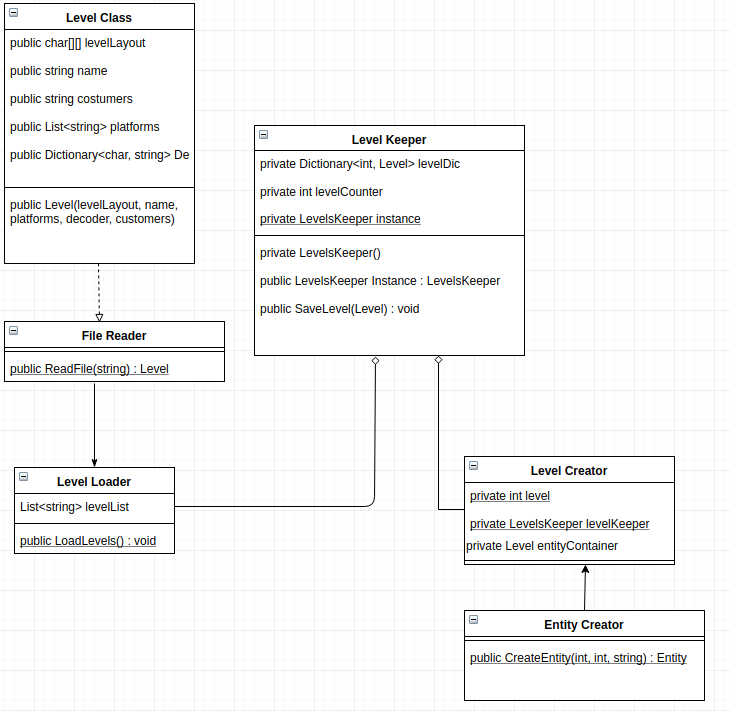
\includegraphics[width=\linewidth]{latex/Images/UML.png}

Som det ses på vores class diagram så er de fleste af vores klasser statiske. Da vi ikke skal bruge flere instanser af for eksempel LevelLoader så vi det mere intuitivt at holde Program og Game fri for objekter som kun skal benyttes en eller få gange, og i stedet bare lade dem kalde statiske metoder i de statiske klasser.\\
Undtagelser på det ovenstående er vores Level class som instatierer et nyt Level objekt. Da vi ønsker at benytte vores Level objekter som en måde at lagre information om vores levels, har vi valgt kun at implementere en konstruktor til dem og ellers gemme alle informationer i public properties uden setters. Dette garanterer at når Level først er blevet instantieret kan dens informationer ikke overskrives, men informationerne kan til enhver tid læses.\\
En anden undtagelse er LevelsKeeper. LevelsKeeper fungerer som en database for vores levels, og indeholder en dictionary af level numre som keys og Level objekter som values. LevelsKeeper er implementeret som en singleton. Dette er gjort for at arbejde med værdier frem for referencer hvilket bevirker at vi ikke skal bekymre os om hvad der sker hvis der læses og skrives til den samme hukommelse samtidigt. Som det fremgik af vores sequence diagram vil dette ikke kunne lade sig gøre med den nuværende implementation, men skulle det blive nødvendigt at udvide vores model med endnu en klasse som skriver til LevelsKeeper samtidigt med at spillet kører, så kan dette sikkert implementeres. Alternativt ville vi kunne have lavet LevelsKeeper static, men så ville vi skulle være sikre på at der aldrig ville skulle skrives og læses det samme sted samtidigt.\\
At LevelsKeeper er en singleton bevirker at både LevelLoader og LevelCreator skal holde en variabel for LevelsKeeper objektet, som kan kalde sine private metoder til at gemme og returnere Level objekter. Disse to metoder er private for at følge princippet om at hver class udfører opgaverne for sit eget ansvar.\\

Som nævnt tidligere vil vi i denne uge antage at alle blokke som danner vores level skal være lige store og have de samme egenskaber. Dette sørger EntityCreator for. I fremtiden vil vi formodentlig skulle gøre forskel på blokke og platforme, og sørge for at de kan have forskellig facon. Dette vil vi nemt kunne indføre i vores design ved at implementere en superklasse hvorfra en platforms klasse og en blokklasse kan arve fra. Det vil da blive EntityCreators opgave at enten kalde en klasse som kan returnere en platform, eller en klasse som kan returnere en blok, afhængigt af oplysningerne fra LevelCreator. På denne måde vil vi nemt kunne udføre collission detection og afgøre om vi har ramt en blok eller en platform.
